\batchmode


\documentclass[english]{article}
\RequirePackage{ifthen}


\usepackage{babel}
\usepackage{supertabular}
\usepackage{html}
\usepackage{times}
\usepackage{graphicx}
\usepackage{hyperref}
\usepackage[T1]{fontenc}

%
\providecommand{\docmttype}{Reference Manual for C}%
\providecommand{\req}[1]{\section{\hspace{.2in}#1}}%
\providecommand{\sreq}[1]{\subsection{\hspace{.2in}#1}}%
\providecommand{\ssreq}[1]{\subsubsection{\hspace{.2in}#1}}%
\providecommand{\mytitle}{ESMF Reference Manual for C~~}%
\providecommand{\myversion}{Version 4.0}
%
\newenvironment{reqlist}{\begin{list} {} {} \rm \item[]}
{\end{list}}
\setcounter{secnumdepth}{3}\setcounter{tocdepth}{3}
%
\providecommand{\longname}{ESMF }%
\providecommand{\funcname}{ESMF }%
\providecommand{\shortname}{REF}%
\providecommand{\myauthors}{ESMF Joint Specification Team:  V. Balaji, Byron Boville, Samson Cheung, Nancy Collins, Tony Craig, Carlos Cruz, Arlindo da Silva, Cecelia DeLuca, Rosalinda de Fainchtein, Brian Eaton, Bob Hallberg, Tom Henderson, Chris Hill, Mark Iredell, Rob Jacob, Phil Jones, Erik Kluzek, Brian Kauffman, Jay Larson, Peggy Li, Fei Liu, John Michalakes, Sylvia Murphy, David Neckels, Ryan O Kuinghttons, Bob Oehmke, Chuck Panaccione, Jim Rosinski, Will Sawyer, Earl Schwab, Shepard Smithline, Walter Spector, Don Stark, Max Suarez, Spencer Swift, Gerhard Theurich, Atanas Trayanov, Silverio Vasquez, Jon Wolfe, Weiyu Yang, Mike Young, Leonid Zaslavsky}\setlength{\textwidth}{6.5truein}\setlength{\textheight}{8.5truein}\setlength{\oddsidemargin}{0in}\setlength{\unitlength}{1truecm}
\hbadness = 10000
\vbadness = 10000



\usepackage[dvips]{color}


\pagecolor[gray]{.7}

\usepackage[]{inputenc}



\makeatletter

\makeatletter
\count@=\the\catcode`\_ \catcode`\_=8 
\newenvironment{tex2html_wrap}{}{}%
\catcode`\<=12\catcode`\_=\count@
\newcommand{\providedcommand}[1]{\expandafter\providecommand\csname #1\endcsname}%
\newcommand{\renewedcommand}[1]{\expandafter\providecommand\csname #1\endcsname{}%
  \expandafter\renewcommand\csname #1\endcsname}%
\newcommand{\newedenvironment}[1]{\newenvironment{#1}{}{}\renewenvironment{#1}}%
\let\newedcommand\renewedcommand
\let\renewedenvironment\newedenvironment
\makeatother
\let\mathon=$
\let\mathoff=$
\ifx\AtBeginDocument\undefined \newcommand{\AtBeginDocument}[1]{}\fi
\newbox\sizebox
\setlength{\hoffset}{0pt}\setlength{\voffset}{0pt}
\addtolength{\textheight}{\footskip}\setlength{\footskip}{0pt}
\addtolength{\textheight}{\topmargin}\setlength{\topmargin}{0pt}
\addtolength{\textheight}{\headheight}\setlength{\headheight}{0pt}
\addtolength{\textheight}{\headsep}\setlength{\headsep}{0pt}
\setlength{\textwidth}{349pt}
\newwrite\lthtmlwrite
\makeatletter
\let\realnormalsize=\normalsize
\global\topskip=2sp
\def\preveqno{}\let\real@float=\@float \let\realend@float=\end@float
\def\@float{\let\@savefreelist\@freelist\real@float}
\def\liih@math{\ifmmode$\else\bad@math\fi}
\def\end@float{\realend@float\global\let\@freelist\@savefreelist}
\let\real@dbflt=\@dbflt \let\end@dblfloat=\end@float
\let\@largefloatcheck=\relax
\let\if@boxedmulticols=\iftrue
\def\@dbflt{\let\@savefreelist\@freelist\real@dbflt}
\def\adjustnormalsize{\def\normalsize{\mathsurround=0pt \realnormalsize
 \parindent=0pt\abovedisplayskip=0pt\belowdisplayskip=0pt}%
 \def\phantompar{\csname par\endcsname}\normalsize}%
\def\lthtmltypeout#1{{\let\protect\string \immediate\write\lthtmlwrite{#1}}}%
\newcommand\lthtmlhboxmathA{\adjustnormalsize\setbox\sizebox=\hbox\bgroup\kern.05em }%
\newcommand\lthtmlhboxmathB{\adjustnormalsize\setbox\sizebox=\hbox to\hsize\bgroup\hfill }%
\newcommand\lthtmlvboxmathA{\adjustnormalsize\setbox\sizebox=\vbox\bgroup %
 \let\ifinner=\iffalse \let\)\liih@math }%
\newcommand\lthtmlboxmathZ{\@next\next\@currlist{}{\def\next{\voidb@x}}%
 \expandafter\box\next\egroup}%
\newcommand\lthtmlmathtype[1]{\gdef\lthtmlmathenv{#1}}%
\newcommand\lthtmllogmath{\lthtmltypeout{l2hSize %
:\lthtmlmathenv:\the\ht\sizebox::\the\dp\sizebox::\the\wd\sizebox.\preveqno}}%
\newcommand\lthtmlfigureA[1]{\let\@savefreelist\@freelist
       \lthtmlmathtype{#1}\lthtmlvboxmathA}%
\newcommand\lthtmlpictureA{\bgroup\catcode`\_=8 \lthtmlpictureB}%
\newcommand\lthtmlpictureB[1]{\lthtmlmathtype{#1}\egroup
       \let\@savefreelist\@freelist \lthtmlhboxmathB}%
\newcommand\lthtmlpictureZ[1]{\hfill\lthtmlfigureZ}%
\newcommand\lthtmlfigureZ{\lthtmlboxmathZ\lthtmllogmath\copy\sizebox
       \global\let\@freelist\@savefreelist}%
\newcommand\lthtmldisplayA{\bgroup\catcode`\_=8 \lthtmldisplayAi}%
\newcommand\lthtmldisplayAi[1]{\lthtmlmathtype{#1}\egroup\lthtmlvboxmathA}%
\newcommand\lthtmldisplayB[1]{\edef\preveqno{(\theequation)}%
  \lthtmldisplayA{#1}\let\@eqnnum\relax}%
\newcommand\lthtmldisplayZ{\lthtmlboxmathZ\lthtmllogmath\lthtmlsetmath}%
\newcommand\lthtmlinlinemathA{\bgroup\catcode`\_=8 \lthtmlinlinemathB}
\newcommand\lthtmlinlinemathB[1]{\lthtmlmathtype{#1}\egroup\lthtmlhboxmathA
  \vrule height1.5ex width0pt }%
\newcommand\lthtmlinlineA{\bgroup\catcode`\_=8 \lthtmlinlineB}%
\newcommand\lthtmlinlineB[1]{\lthtmlmathtype{#1}\egroup\lthtmlhboxmathA}%
\newcommand\lthtmlinlineZ{\egroup\expandafter\ifdim\dp\sizebox>0pt %
  \expandafter\centerinlinemath\fi\lthtmllogmath\lthtmlsetinline}
\newcommand\lthtmlinlinemathZ{\egroup\expandafter\ifdim\dp\sizebox>0pt %
  \expandafter\centerinlinemath\fi\lthtmllogmath\lthtmlsetmath}
\newcommand\lthtmlindisplaymathZ{\egroup %
  \centerinlinemath\lthtmllogmath\lthtmlsetmath}
\def\lthtmlsetinline{\hbox{\vrule width.1em \vtop{\vbox{%
  \kern.1em\copy\sizebox}\ifdim\dp\sizebox>0pt\kern.1em\else\kern.3pt\fi
  \ifdim\hsize>\wd\sizebox \hrule depth1pt\fi}}}
\def\lthtmlsetmath{\hbox{\vrule width.1em\kern-.05em\vtop{\vbox{%
  \kern.1em\kern0.8 pt\hbox{\hglue.17em\copy\sizebox\hglue0.8 pt}}\kern.3pt%
  \ifdim\dp\sizebox>0pt\kern.1em\fi \kern0.8 pt%
  \ifdim\hsize>\wd\sizebox \hrule depth1pt\fi}}}
\def\centerinlinemath{%
  \dimen1=\ifdim\ht\sizebox<\dp\sizebox \dp\sizebox\else\ht\sizebox\fi
  \advance\dimen1by.5pt \vrule width0pt height\dimen1 depth\dimen1 
 \dp\sizebox=\dimen1\ht\sizebox=\dimen1\relax}

\def\lthtmlcheckvsize{\ifdim\ht\sizebox<\vsize 
  \ifdim\wd\sizebox<\hsize\expandafter\hfill\fi \expandafter\vfill
  \else\expandafter\vss\fi}%
\providecommand{\selectlanguage}[1]{}%
\makeatletter \tracingstats = 1 


\begin{document}
\pagestyle{empty}\thispagestyle{empty}\lthtmltypeout{}%
\lthtmltypeout{latex2htmlLength hsize=\the\hsize}\lthtmltypeout{}%
\lthtmltypeout{latex2htmlLength vsize=\the\vsize}\lthtmltypeout{}%
\lthtmltypeout{latex2htmlLength hoffset=\the\hoffset}\lthtmltypeout{}%
\lthtmltypeout{latex2htmlLength voffset=\the\voffset}\lthtmltypeout{}%
\lthtmltypeout{latex2htmlLength topmargin=\the\topmargin}\lthtmltypeout{}%
\lthtmltypeout{latex2htmlLength topskip=\the\topskip}\lthtmltypeout{}%
\lthtmltypeout{latex2htmlLength headheight=\the\headheight}\lthtmltypeout{}%
\lthtmltypeout{latex2htmlLength headsep=\the\headsep}\lthtmltypeout{}%
\lthtmltypeout{latex2htmlLength parskip=\the\parskip}\lthtmltypeout{}%
\lthtmltypeout{latex2htmlLength oddsidemargin=\the\oddsidemargin}\lthtmltypeout{}%
\makeatletter
\if@twoside\lthtmltypeout{latex2htmlLength evensidemargin=\the\evensidemargin}%
\else\lthtmltypeout{latex2htmlLength evensidemargin=\the\oddsidemargin}\fi%
\lthtmltypeout{}%
\makeatother
\setcounter{page}{1}
\onecolumn

% !!! IMAGES START HERE !!!

\setcounter{secnumdepth}{3}
\setcounter{tocdepth}{3}
\stepcounter{part}
\stepcounter{section}
\stepcounter{section}
{\newpage\clearpage
\lthtmlpictureA{tex2html_wrap258}%
\scalebox{1.0}{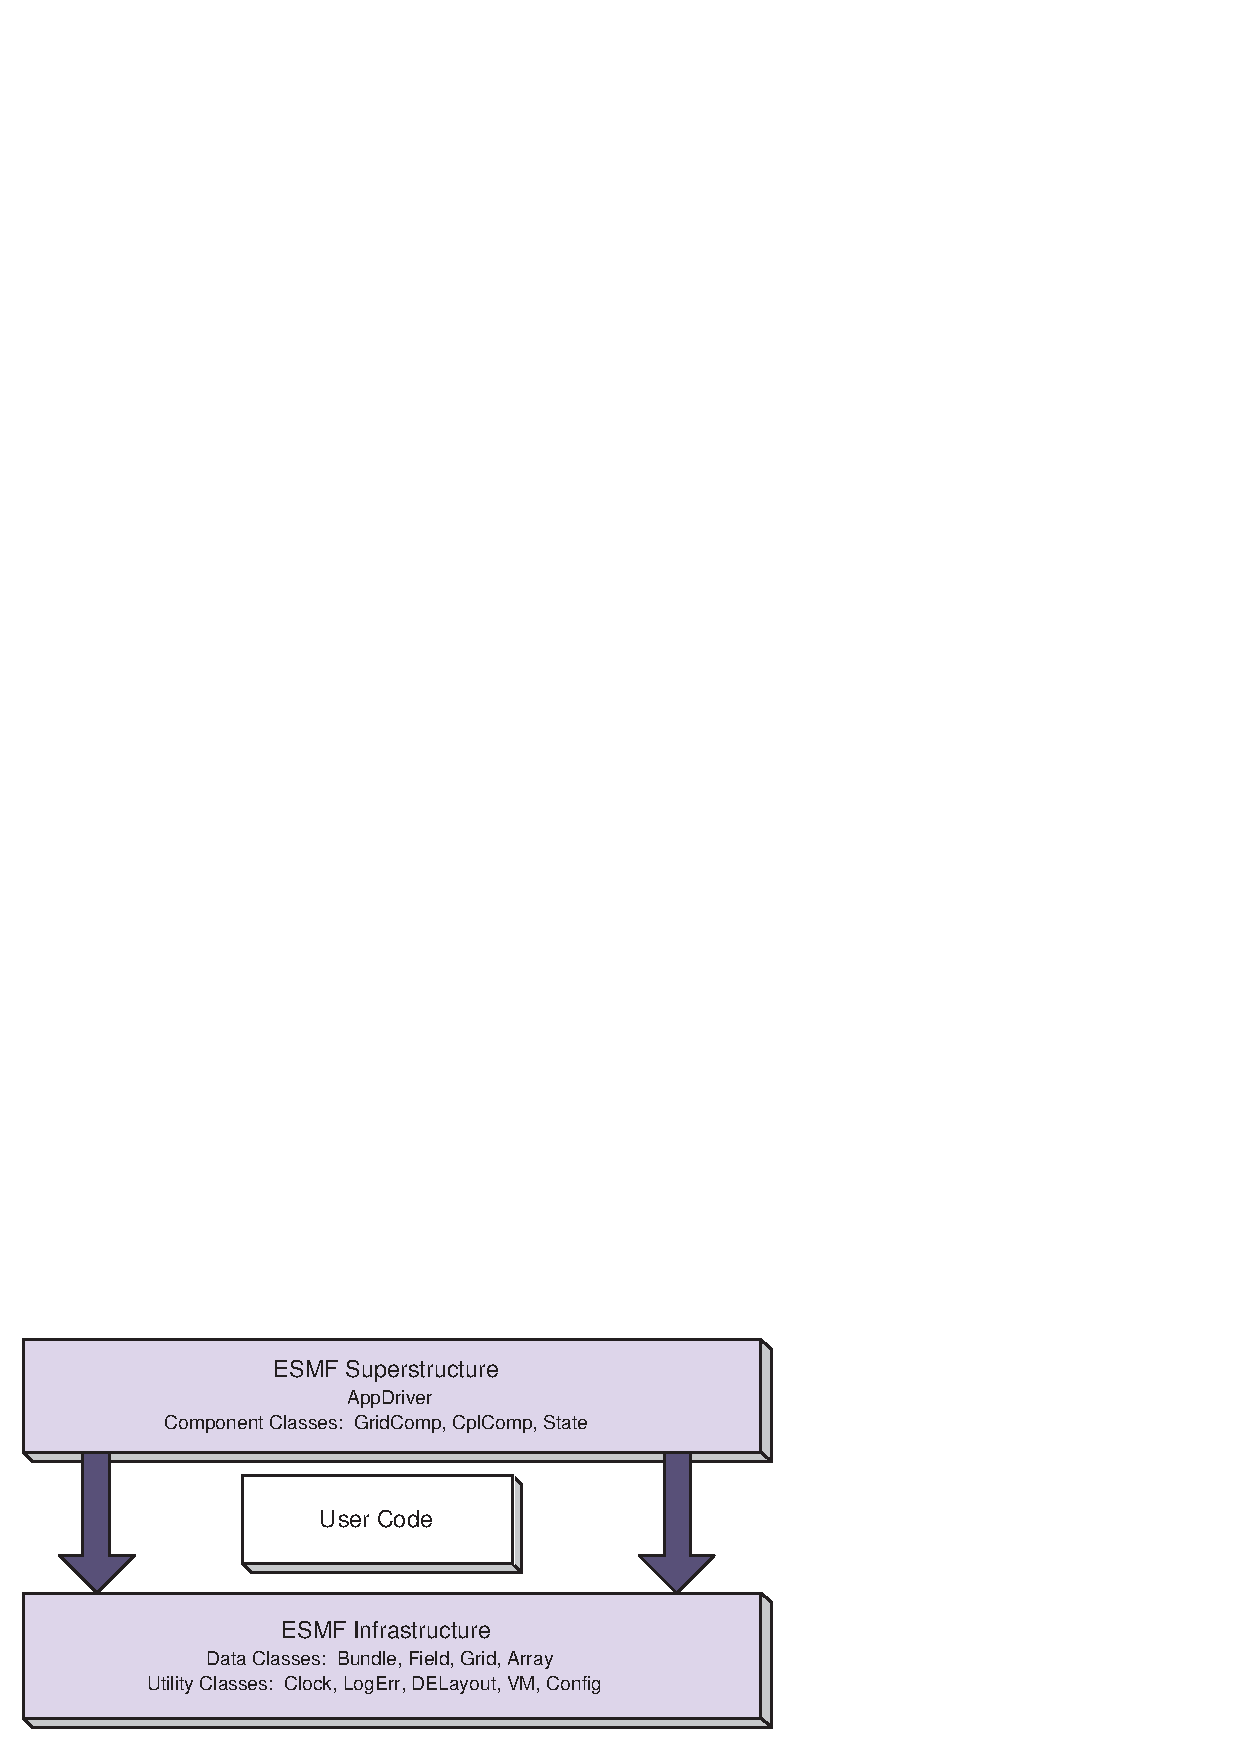
\includegraphics{ESMF_sandwich}}%
\lthtmlpictureZ
\lthtmlcheckvsize\clearpage}

\stepcounter{part}
\stepcounter{section}
\stepcounter{subsection}
{\newpage\clearpage
\lthtmlpictureA{tex2html_wrap424}%
\scalebox{1.0}{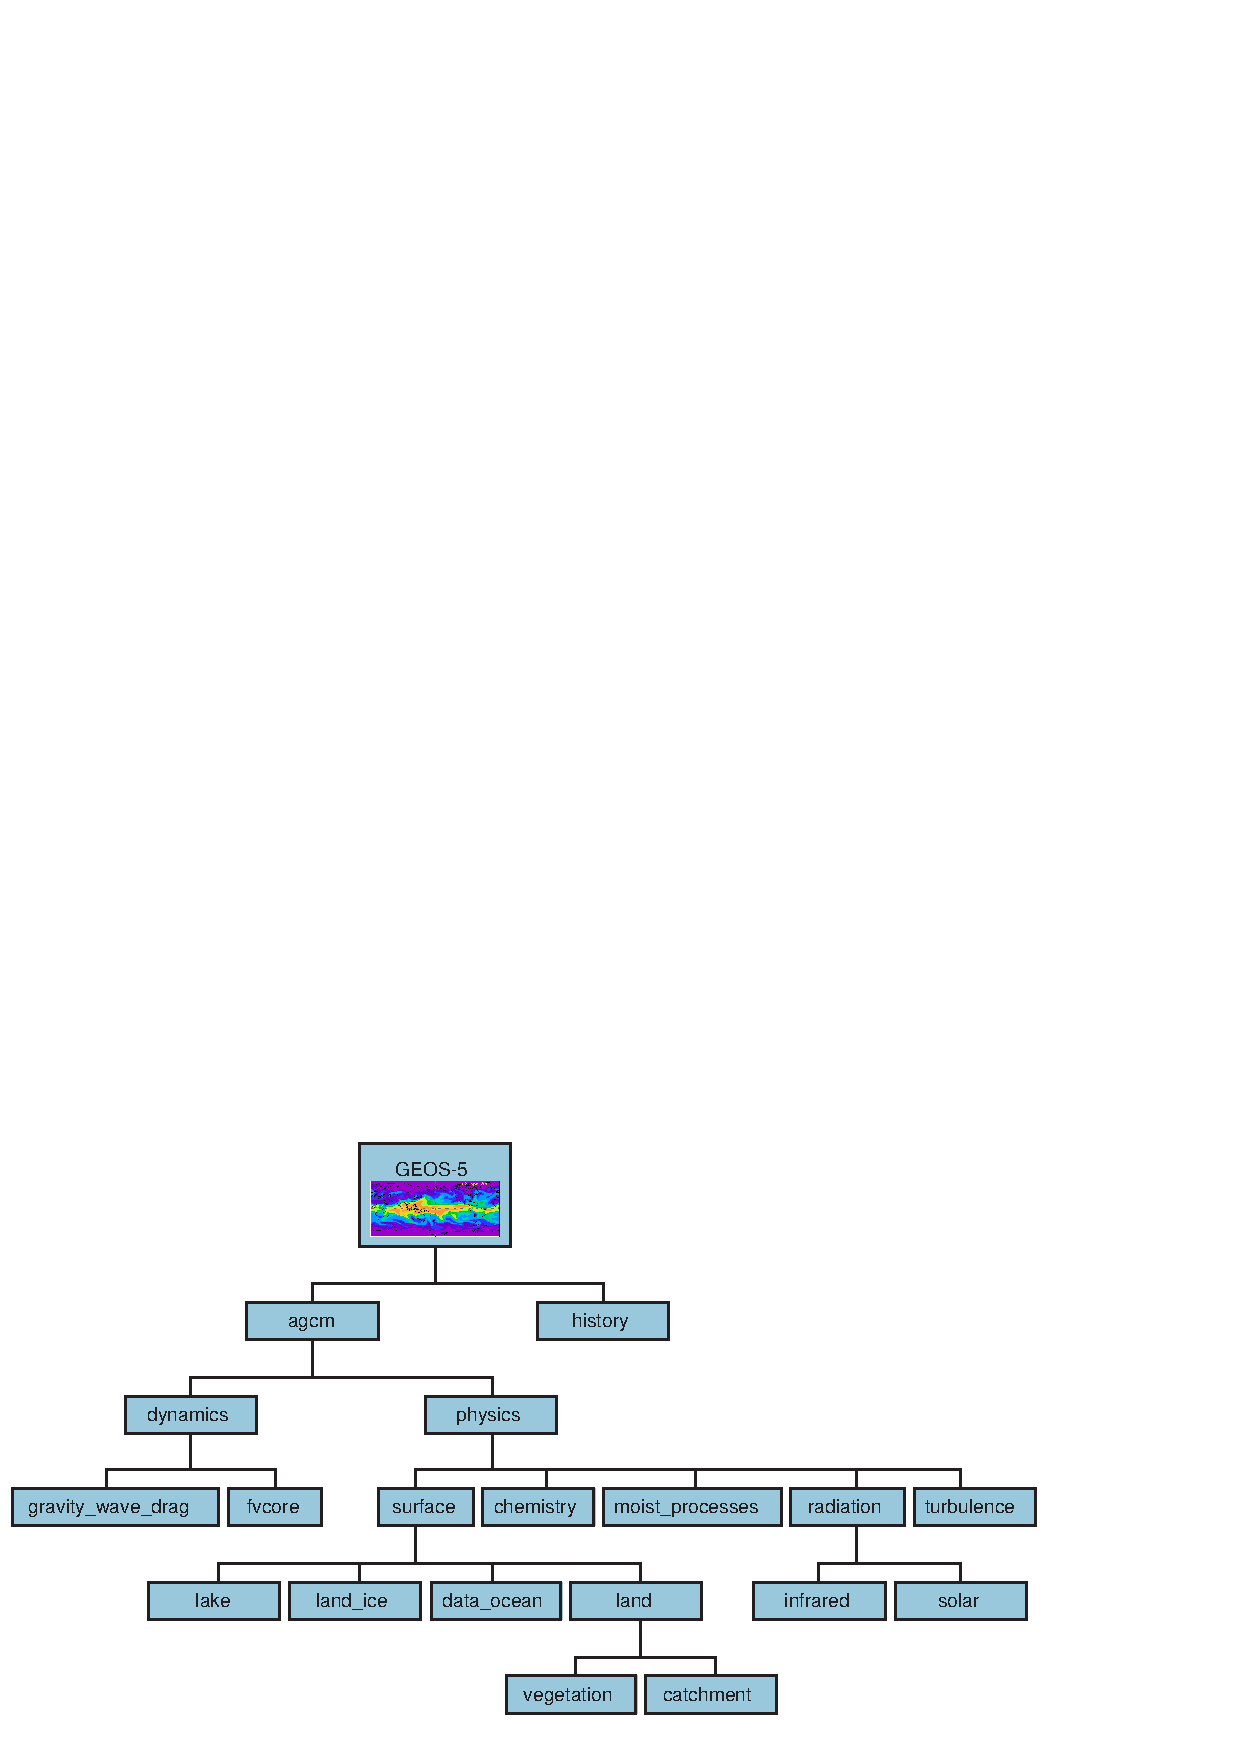
\includegraphics{ESMF_GEOS5}}%
\lthtmlpictureZ
\lthtmlcheckvsize\clearpage}

\stepcounter{subsection}
{\newpage\clearpage
\lthtmlpictureA{tex2html_wrap444}%
\scalebox{1.0}{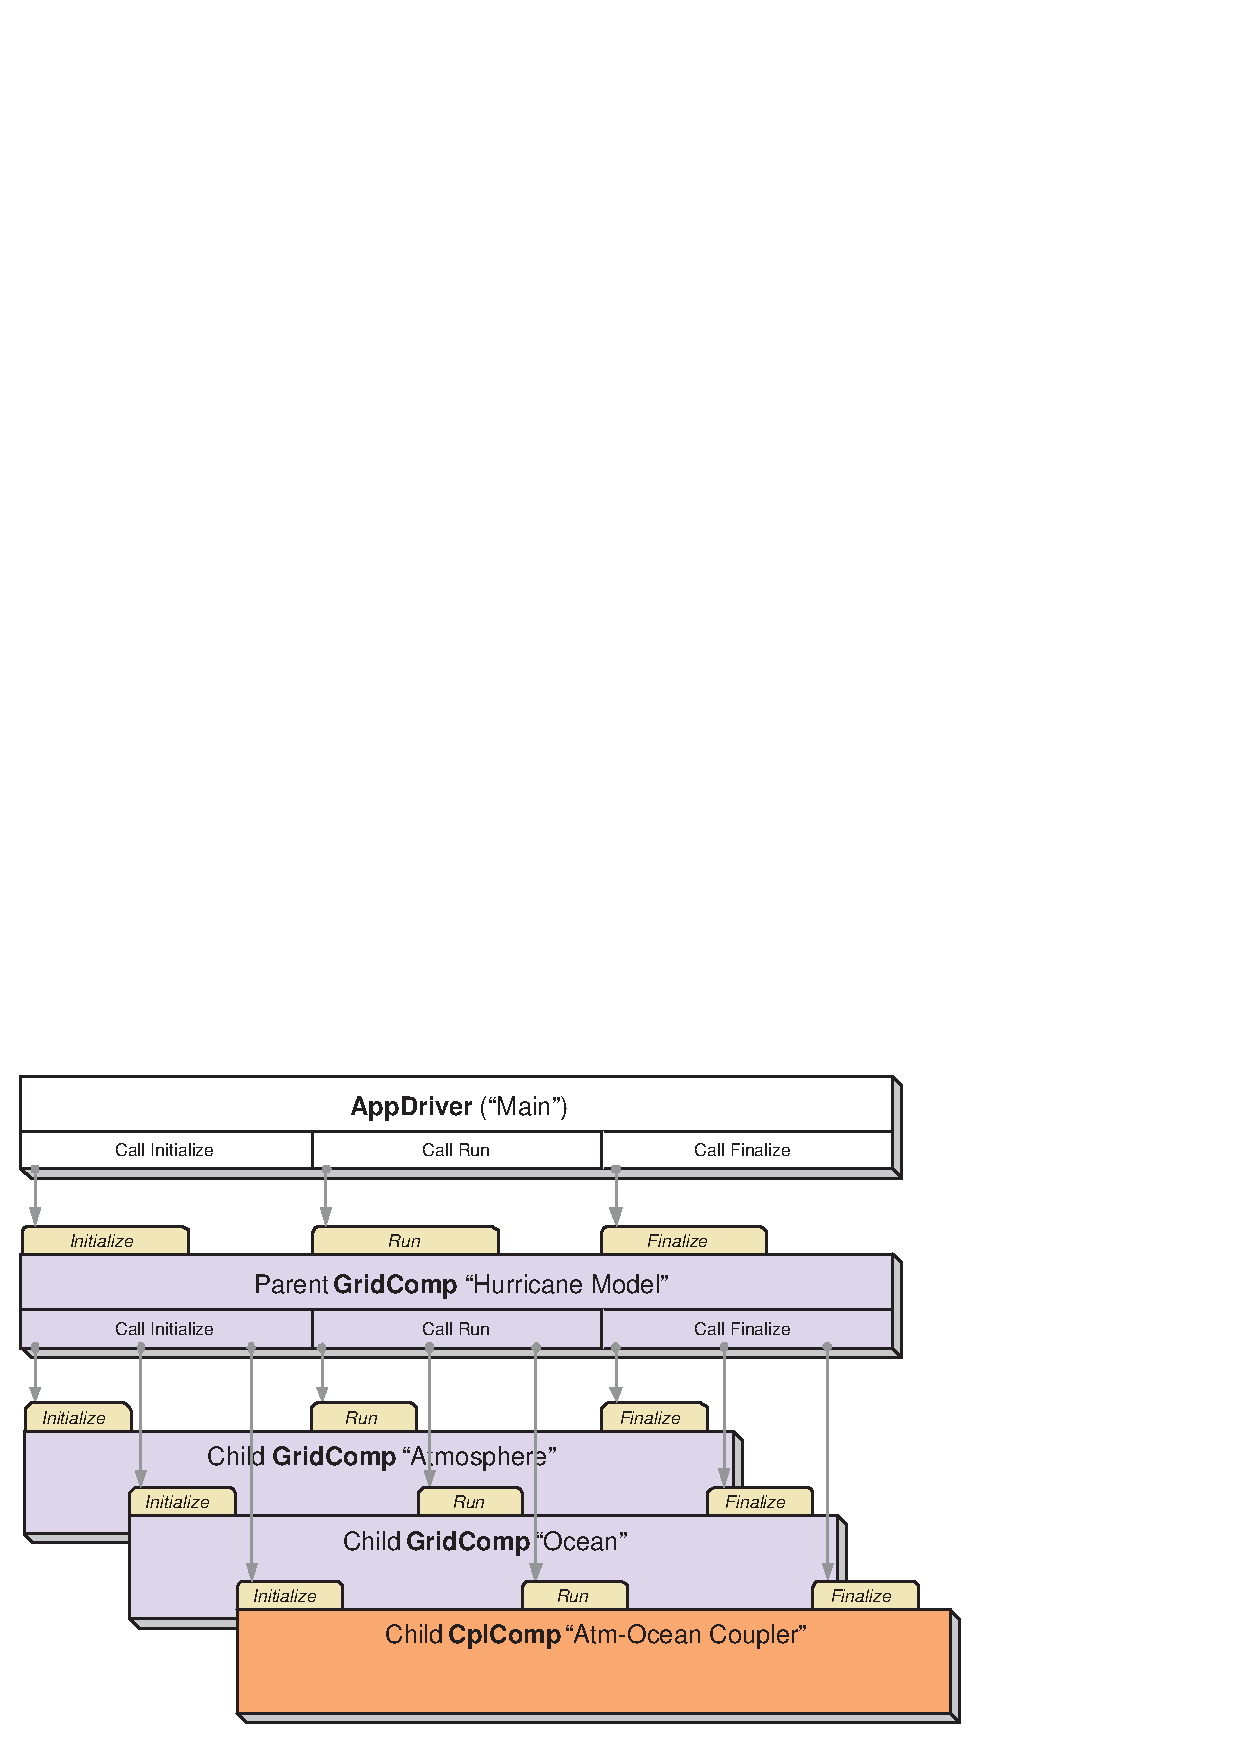
\includegraphics{ESMF_appunit}}%
\lthtmlpictureZ
\lthtmlcheckvsize\clearpage}

\stepcounter{subsection}
{\newpage\clearpage
\lthtmlpictureA{tex2html_wrap464}%
\scalebox{1.0}{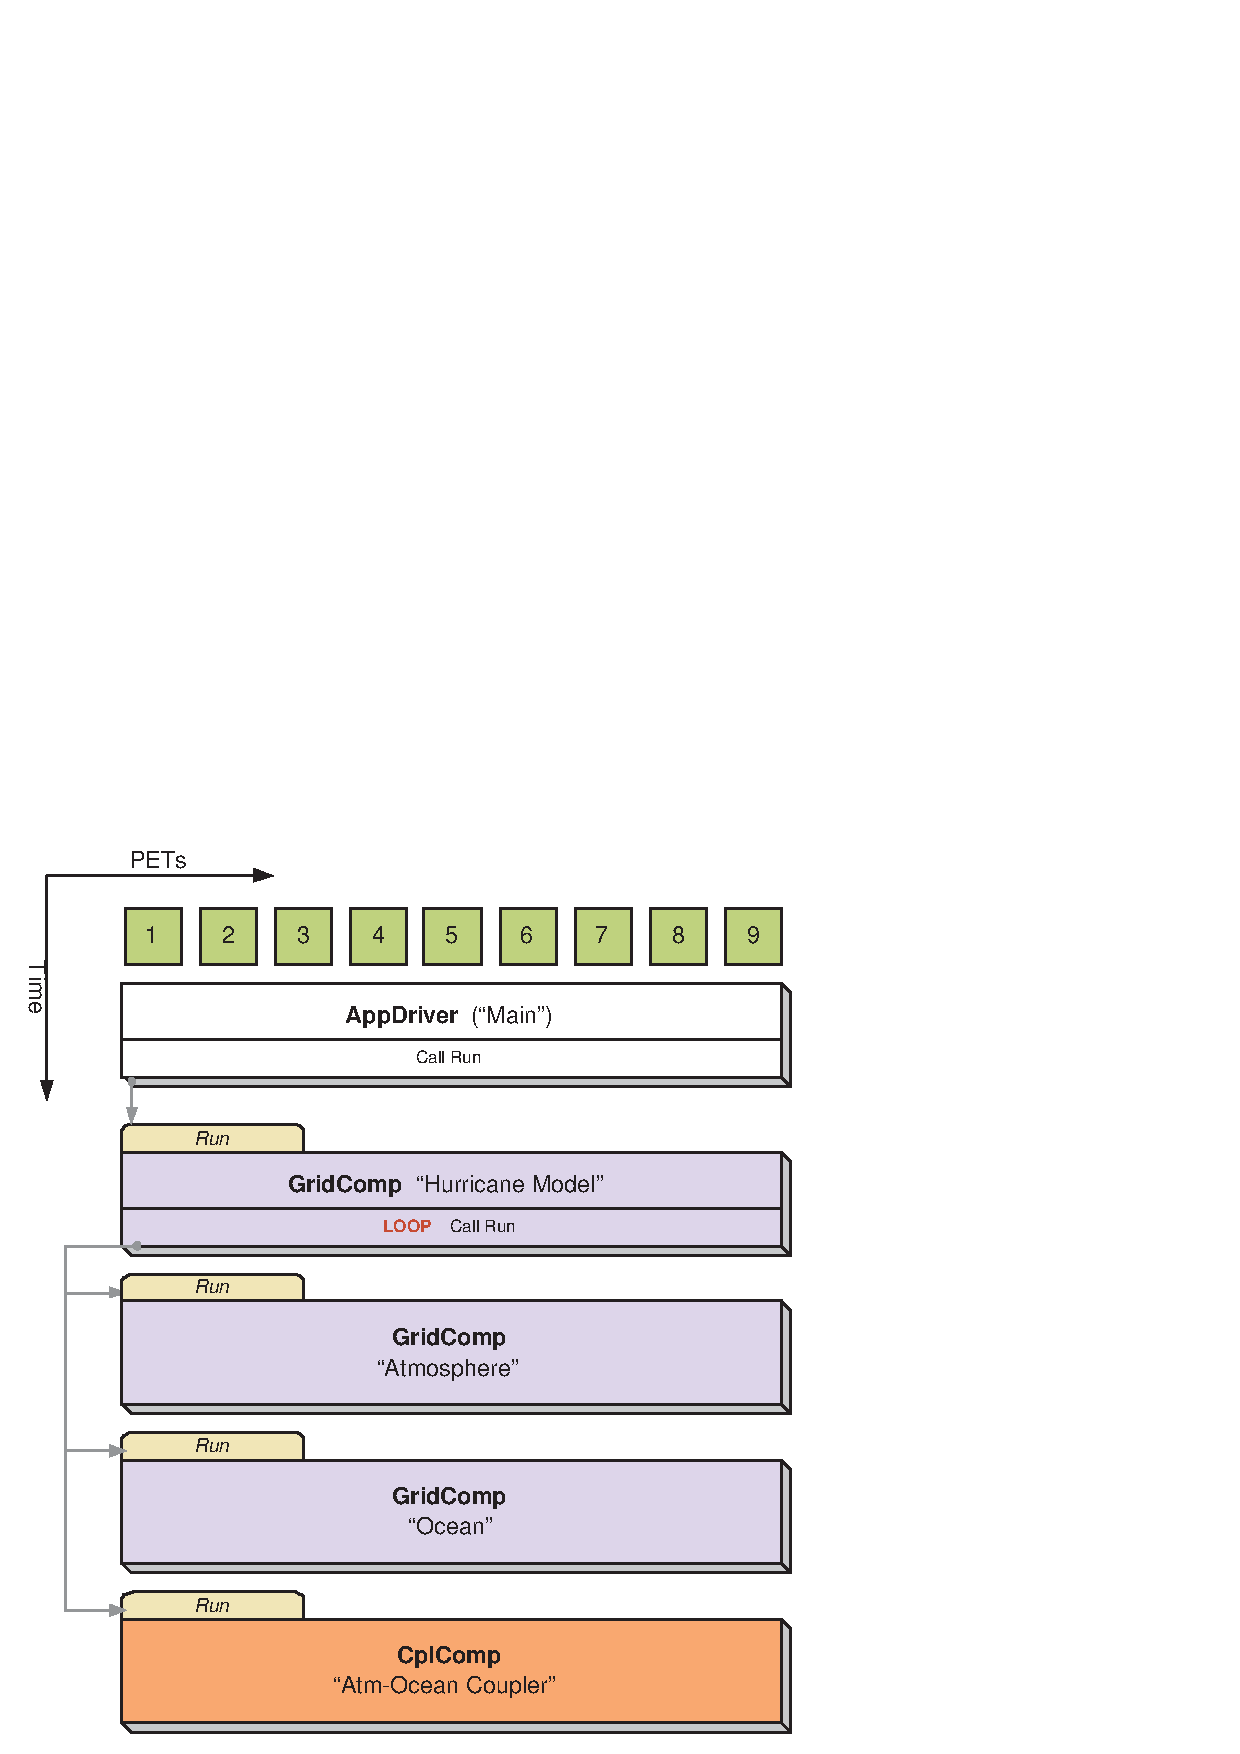
\includegraphics{ESMF_serial}}%
\lthtmlpictureZ
\lthtmlcheckvsize\clearpage}

{\newpage\clearpage
\lthtmlpictureA{tex2html_wrap470}%
\scalebox{1.0}{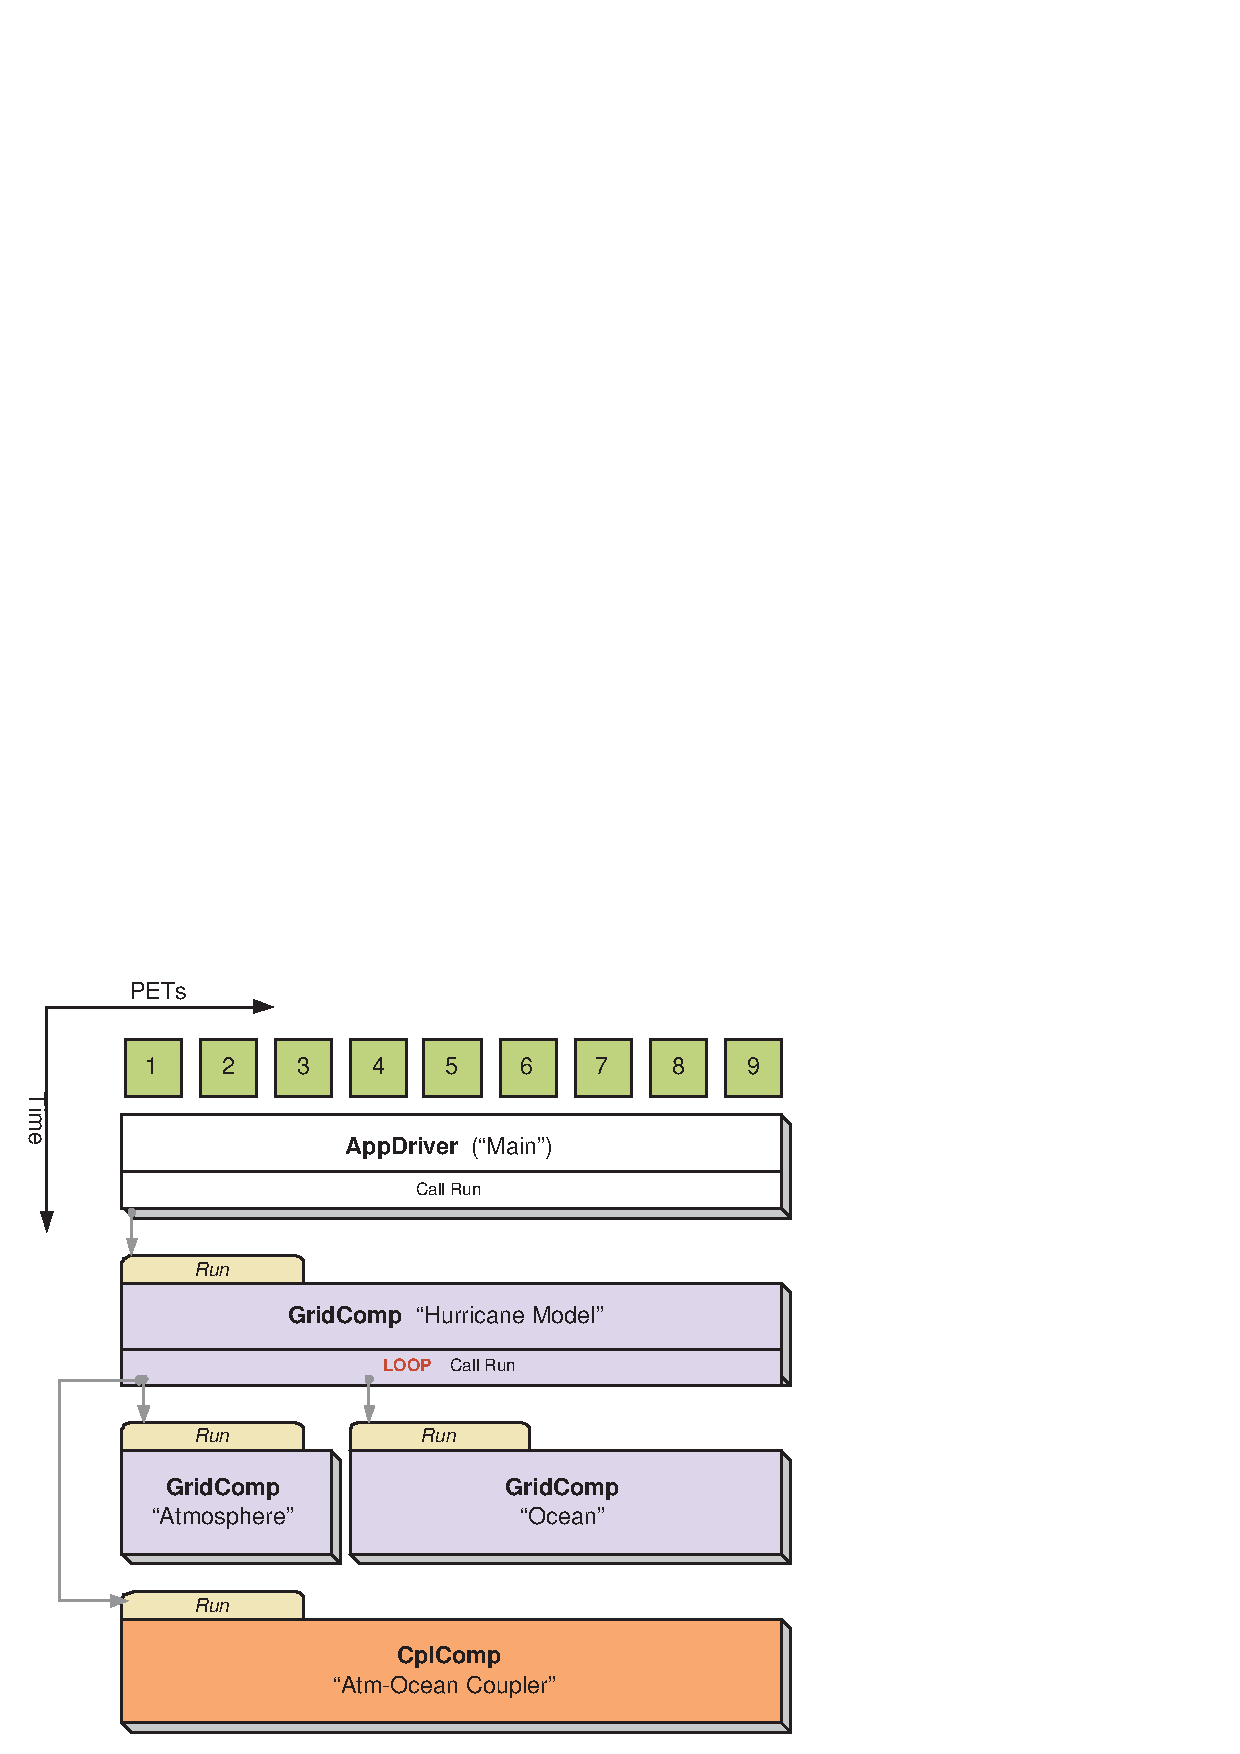
\includegraphics{ESMF_concurrent}}%
\lthtmlpictureZ
\lthtmlcheckvsize\clearpage}

\stepcounter{subsection}
\stepcounter{subsection}
{\newpage\clearpage
\lthtmlpictureA{tex2html_wrap490}%
\scalebox{1.0}{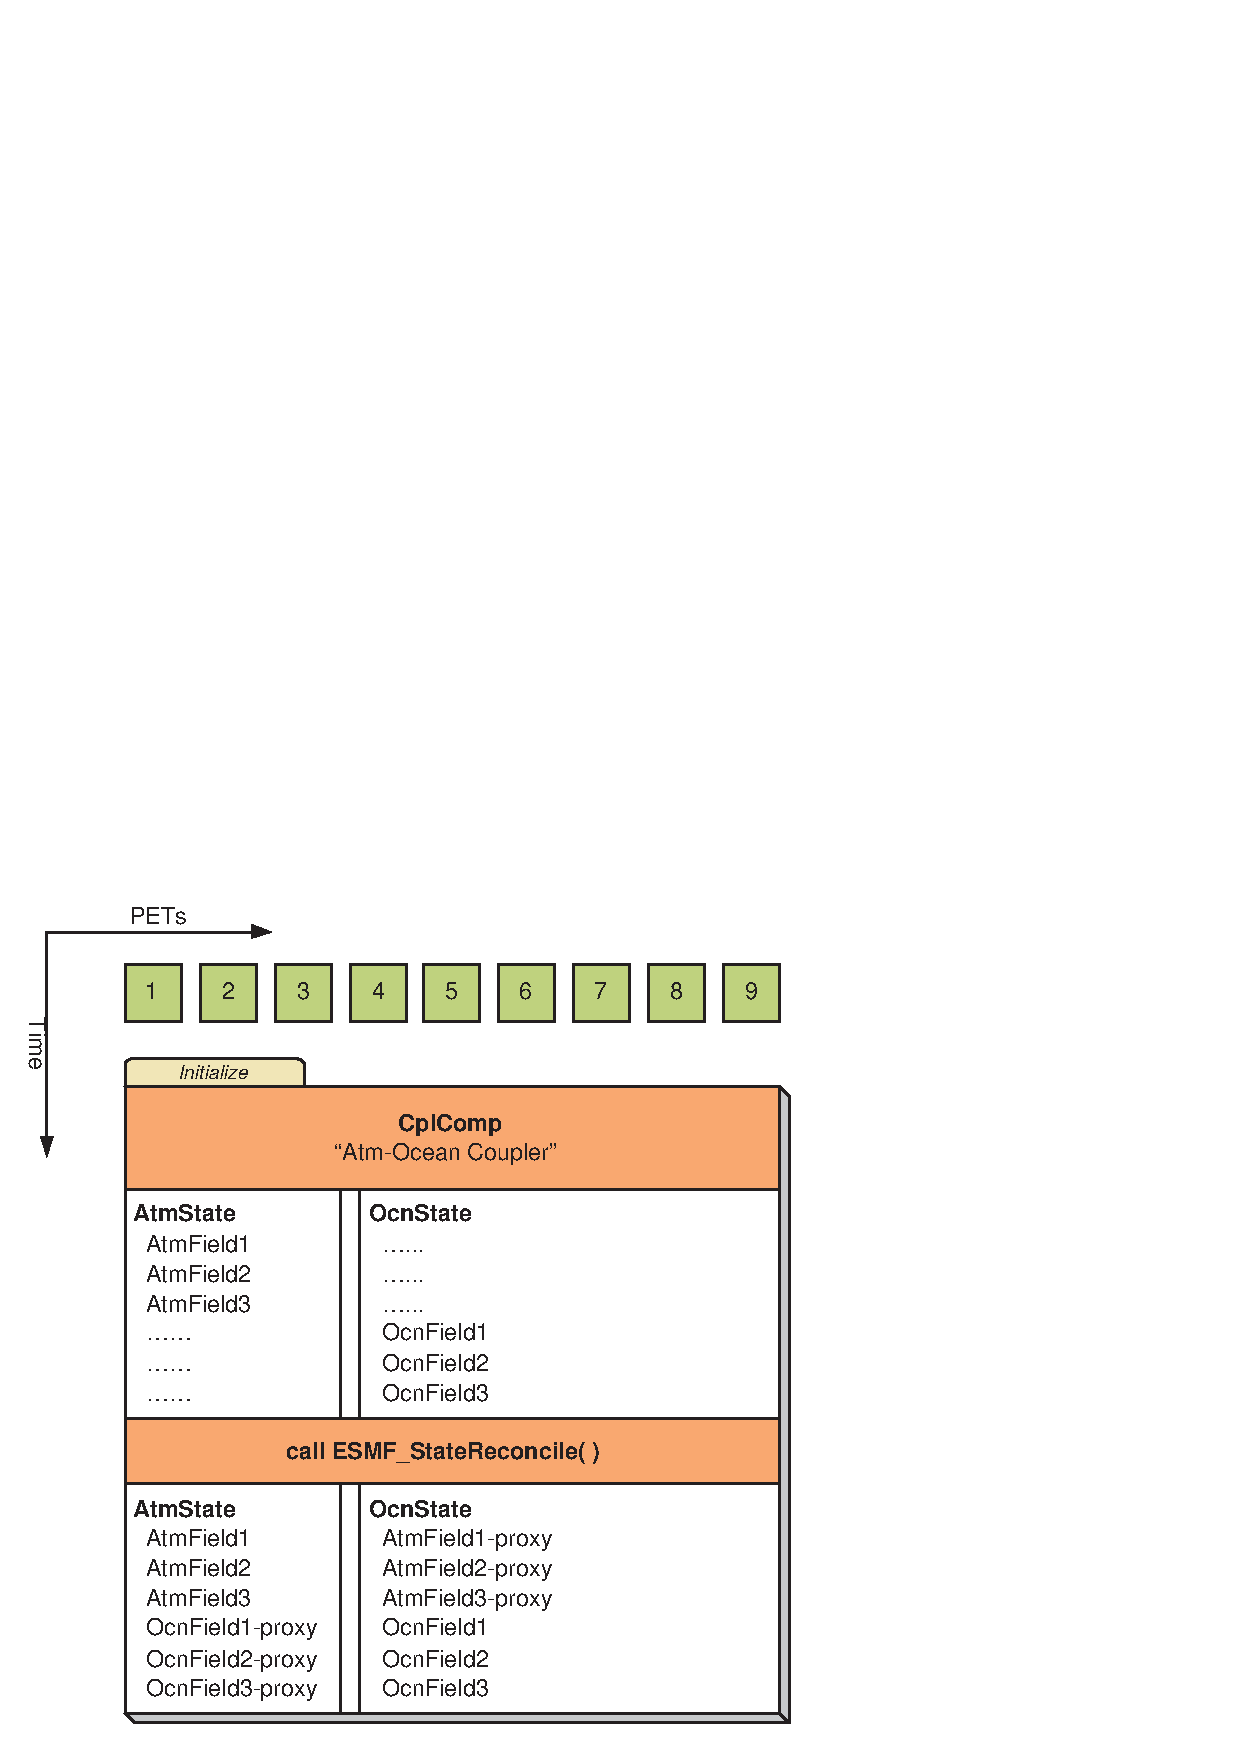
\includegraphics{ESMF_reconcile}}%
\lthtmlpictureZ
\lthtmlcheckvsize\clearpage}

\stepcounter{subsection}
\stepcounter{subsection}
{\newpage\clearpage
\lthtmlpictureA{tex2html_wrap5547}%
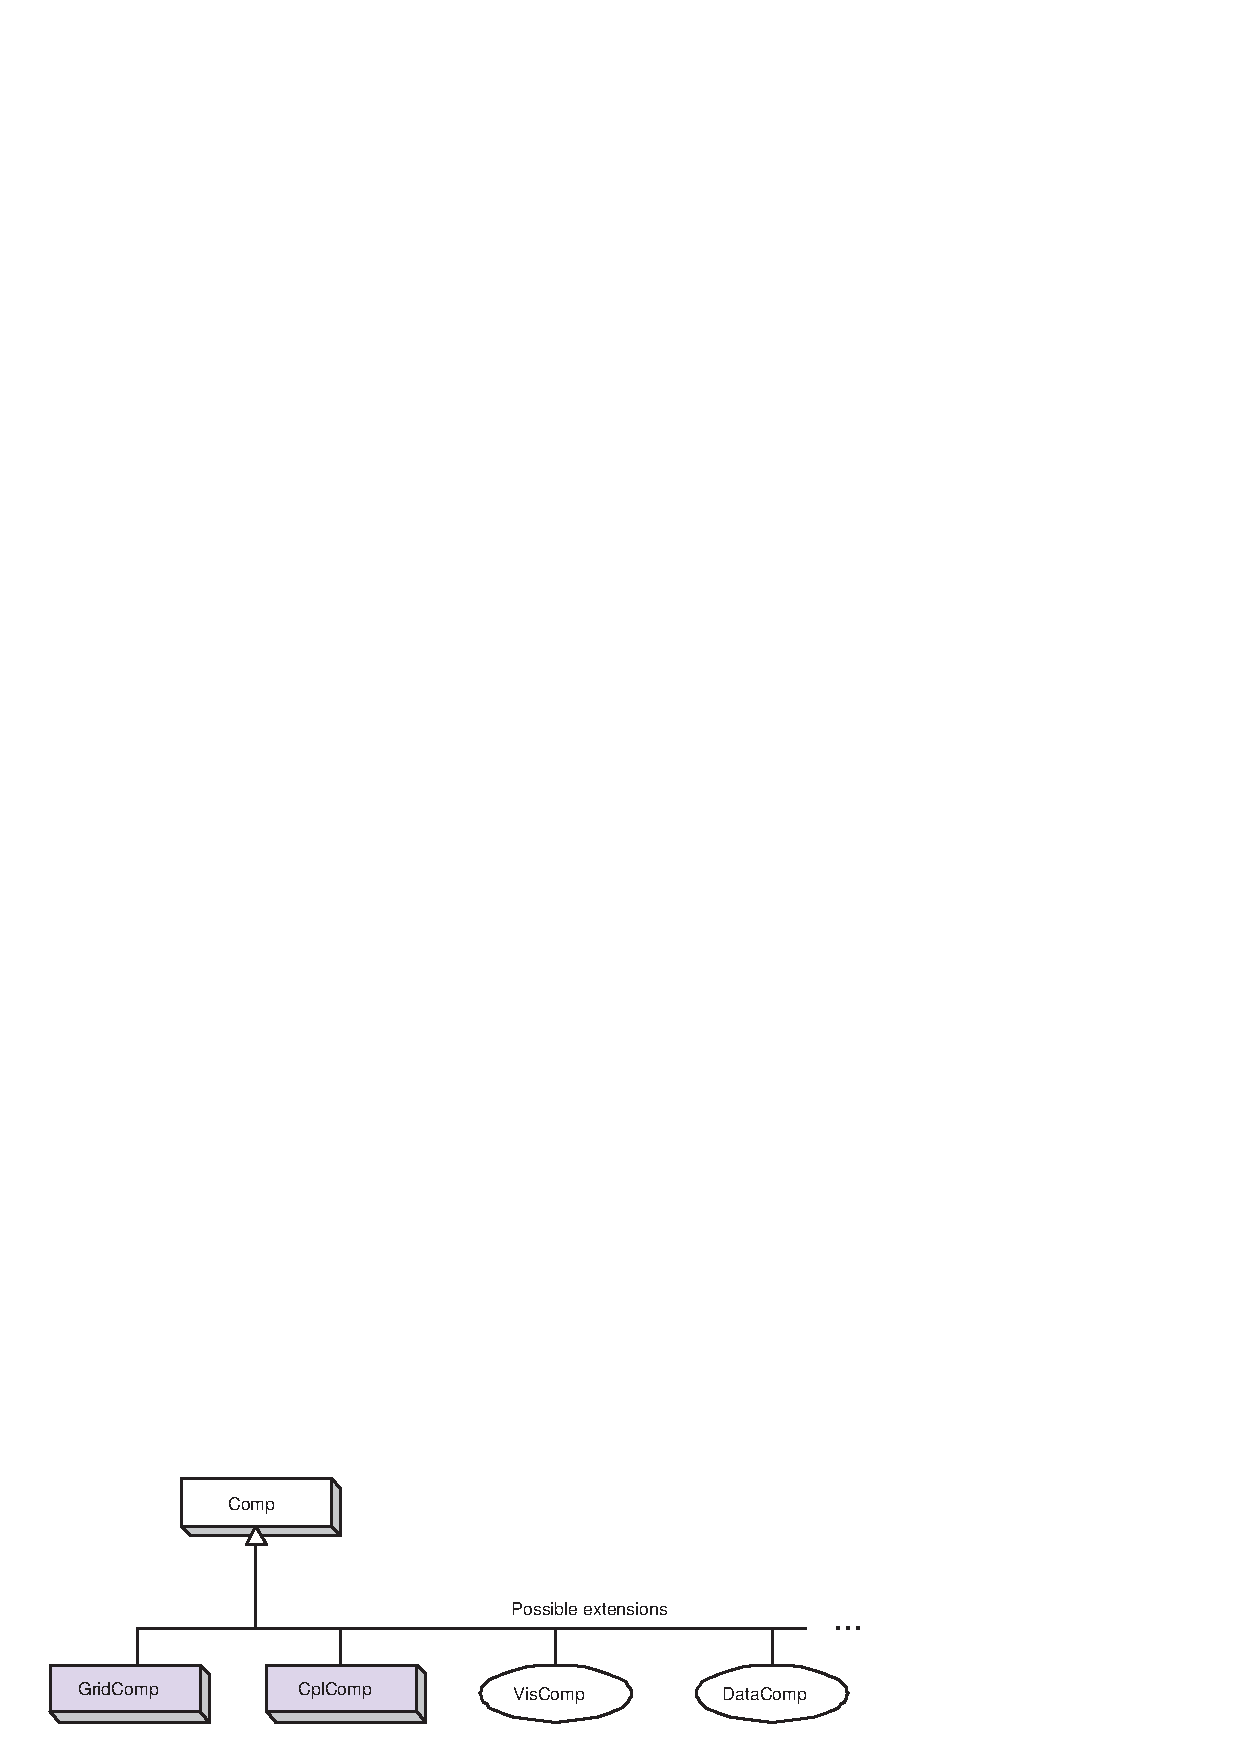
\includegraphics[]{Comp_obj}%
\lthtmlpictureZ
\lthtmlcheckvsize\clearpage}

\stepcounter{section}
\stepcounter{subsection}
\stepcounter{subsection}

\setlength{\parskip}{0pt}%

\setlength{\parskip}{0pt}

\setlength{\parindent}{0pt}%

\setlength{\parindent}{0pt}

\setlength{\baselineskip}{11pt}%

\setlength{\baselineskip}{11pt}
\stepcounter{subsubsection}
\stepcounter{section}
\stepcounter{subsection}
\stepcounter{subsection}

\setlength{\parskip}{0pt}%

\setlength{\parskip}{0pt}

\setlength{\parindent}{0pt}%

\setlength{\parindent}{0pt}

\setlength{\baselineskip}{11pt}%

\setlength{\baselineskip}{11pt}
\stepcounter{subsection}
\stepcounter{section}
\stepcounter{subsection}
\stepcounter{section}
\stepcounter{subsection}
\stepcounter{subsection}

\setlength{\parskip}{0pt}%

\setlength{\parskip}{0pt}

\setlength{\parindent}{0pt}%

\setlength{\parindent}{0pt}

\setlength{\baselineskip}{11pt}%

\setlength{\baselineskip}{11pt}
\stepcounter{subsection}
\stepcounter{part}
\stepcounter{section}
\stepcounter{subsection}
\stepcounter{subsection}
\stepcounter{section}
\stepcounter{subsection}
\stepcounter{subsubsection}
\stepcounter{subsection}

\setlength{\parskip}{0pt}%

\setlength{\parskip}{0pt}

\setlength{\parindent}{0pt}%

\setlength{\parindent}{0pt}

\setlength{\baselineskip}{11pt}%

\setlength{\baselineskip}{11pt}
\stepcounter{subsection}
\stepcounter{section}
\stepcounter{subsection}
\stepcounter{subsection}

\setlength{\parskip}{0pt}%

\setlength{\parskip}{0pt}

\setlength{\parindent}{0pt}%

\setlength{\parindent}{0pt}

\setlength{\baselineskip}{11pt}%

\setlength{\baselineskip}{11pt}
\stepcounter{subsection}
\stepcounter{section}
\stepcounter{subsection}
\stepcounter{subsection}

\setlength{\parskip}{0pt}%

\setlength{\parskip}{0pt}

\setlength{\parindent}{0pt}%

\setlength{\parindent}{0pt}

\setlength{\baselineskip}{11pt}%

\setlength{\baselineskip}{11pt}
\stepcounter{subsection}
\stepcounter{section}
\stepcounter{subsection}
\stepcounter{subsubsection}
\stepcounter{subsubsection}
\stepcounter{subsubsection}
\stepcounter{subsubsection}
{\newpage\clearpage
\lthtmlpictureA{tex2html_wrap1634}%
\scalebox{0.9}{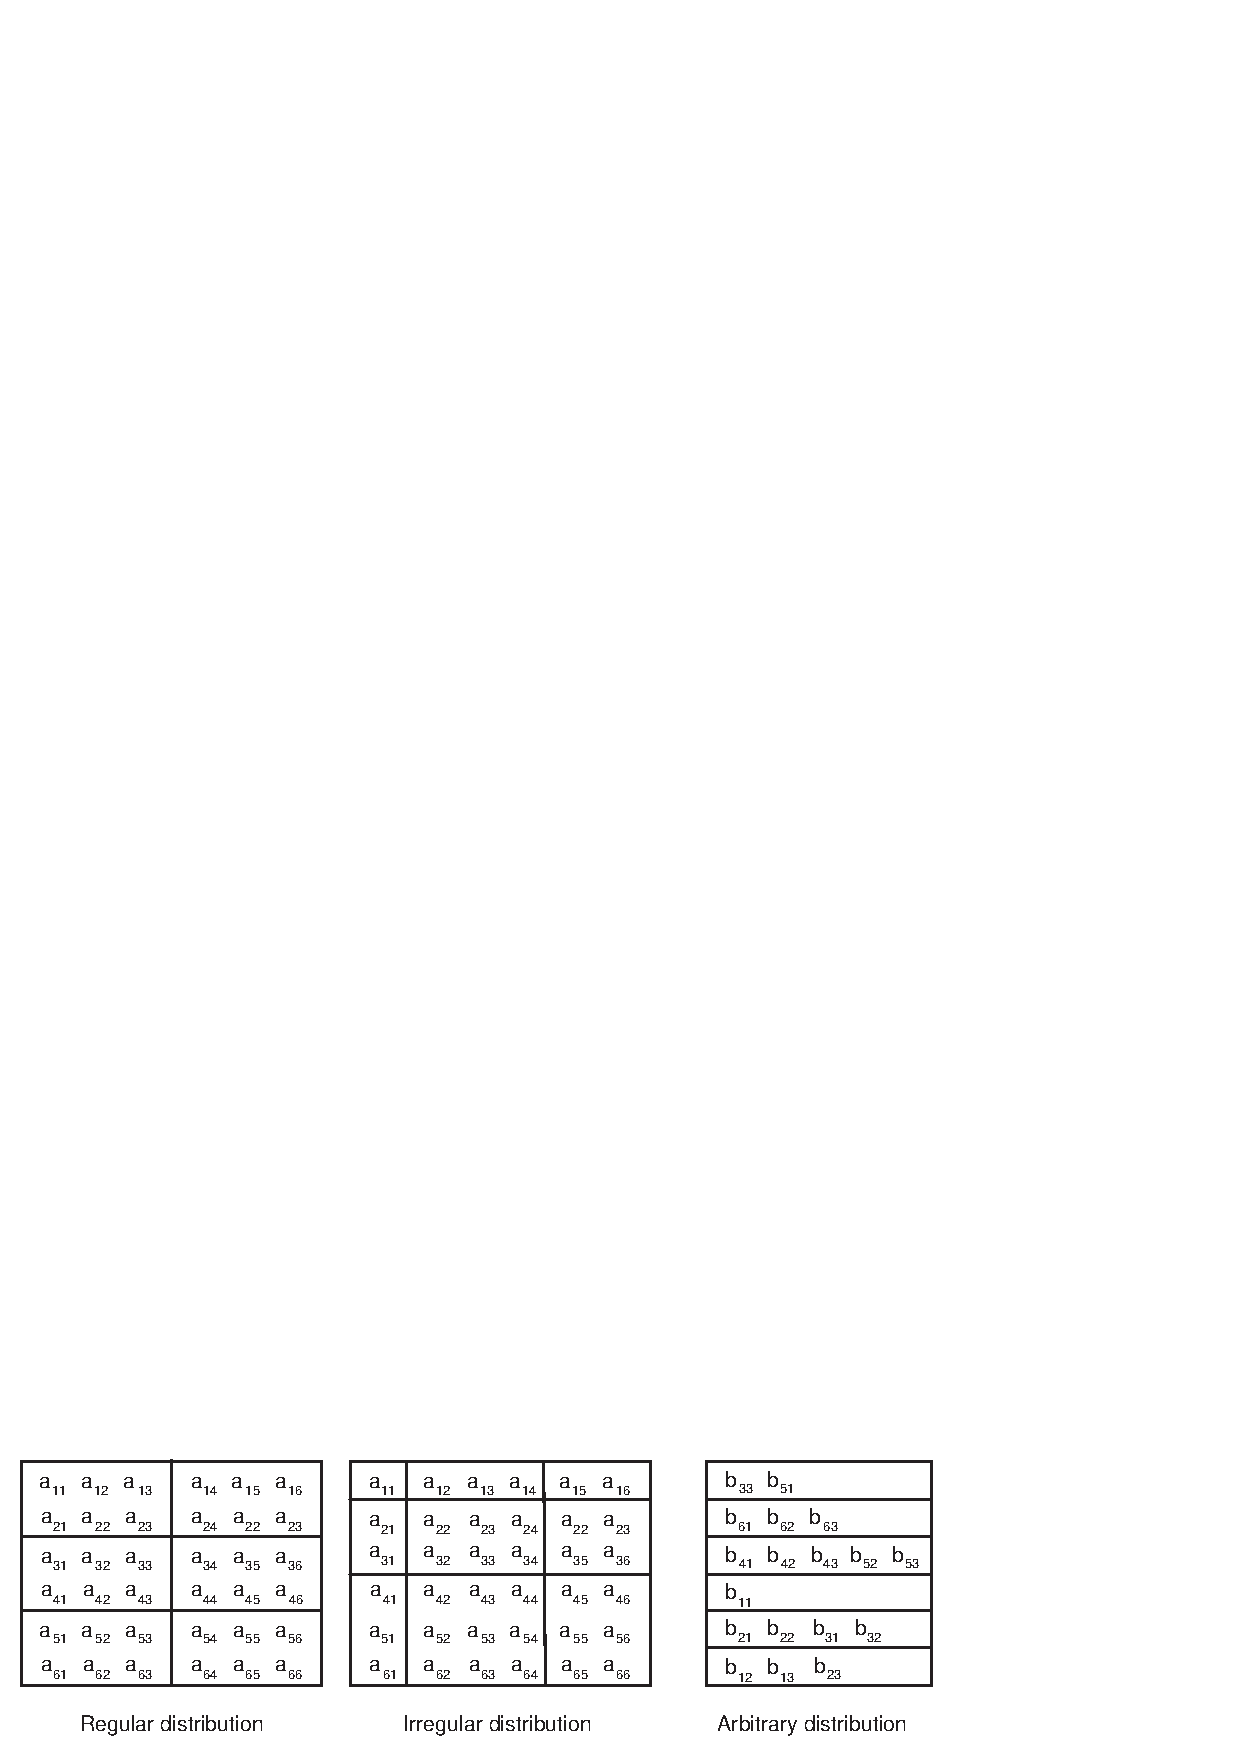
\includegraphics{GridDecomps}}%
\lthtmlpictureZ
\lthtmlcheckvsize\clearpage}

\stepcounter{subsubsection}
{\newpage\clearpage
\lthtmlpictureA{tex2html_wrap1652}%
\scalebox{0.9}{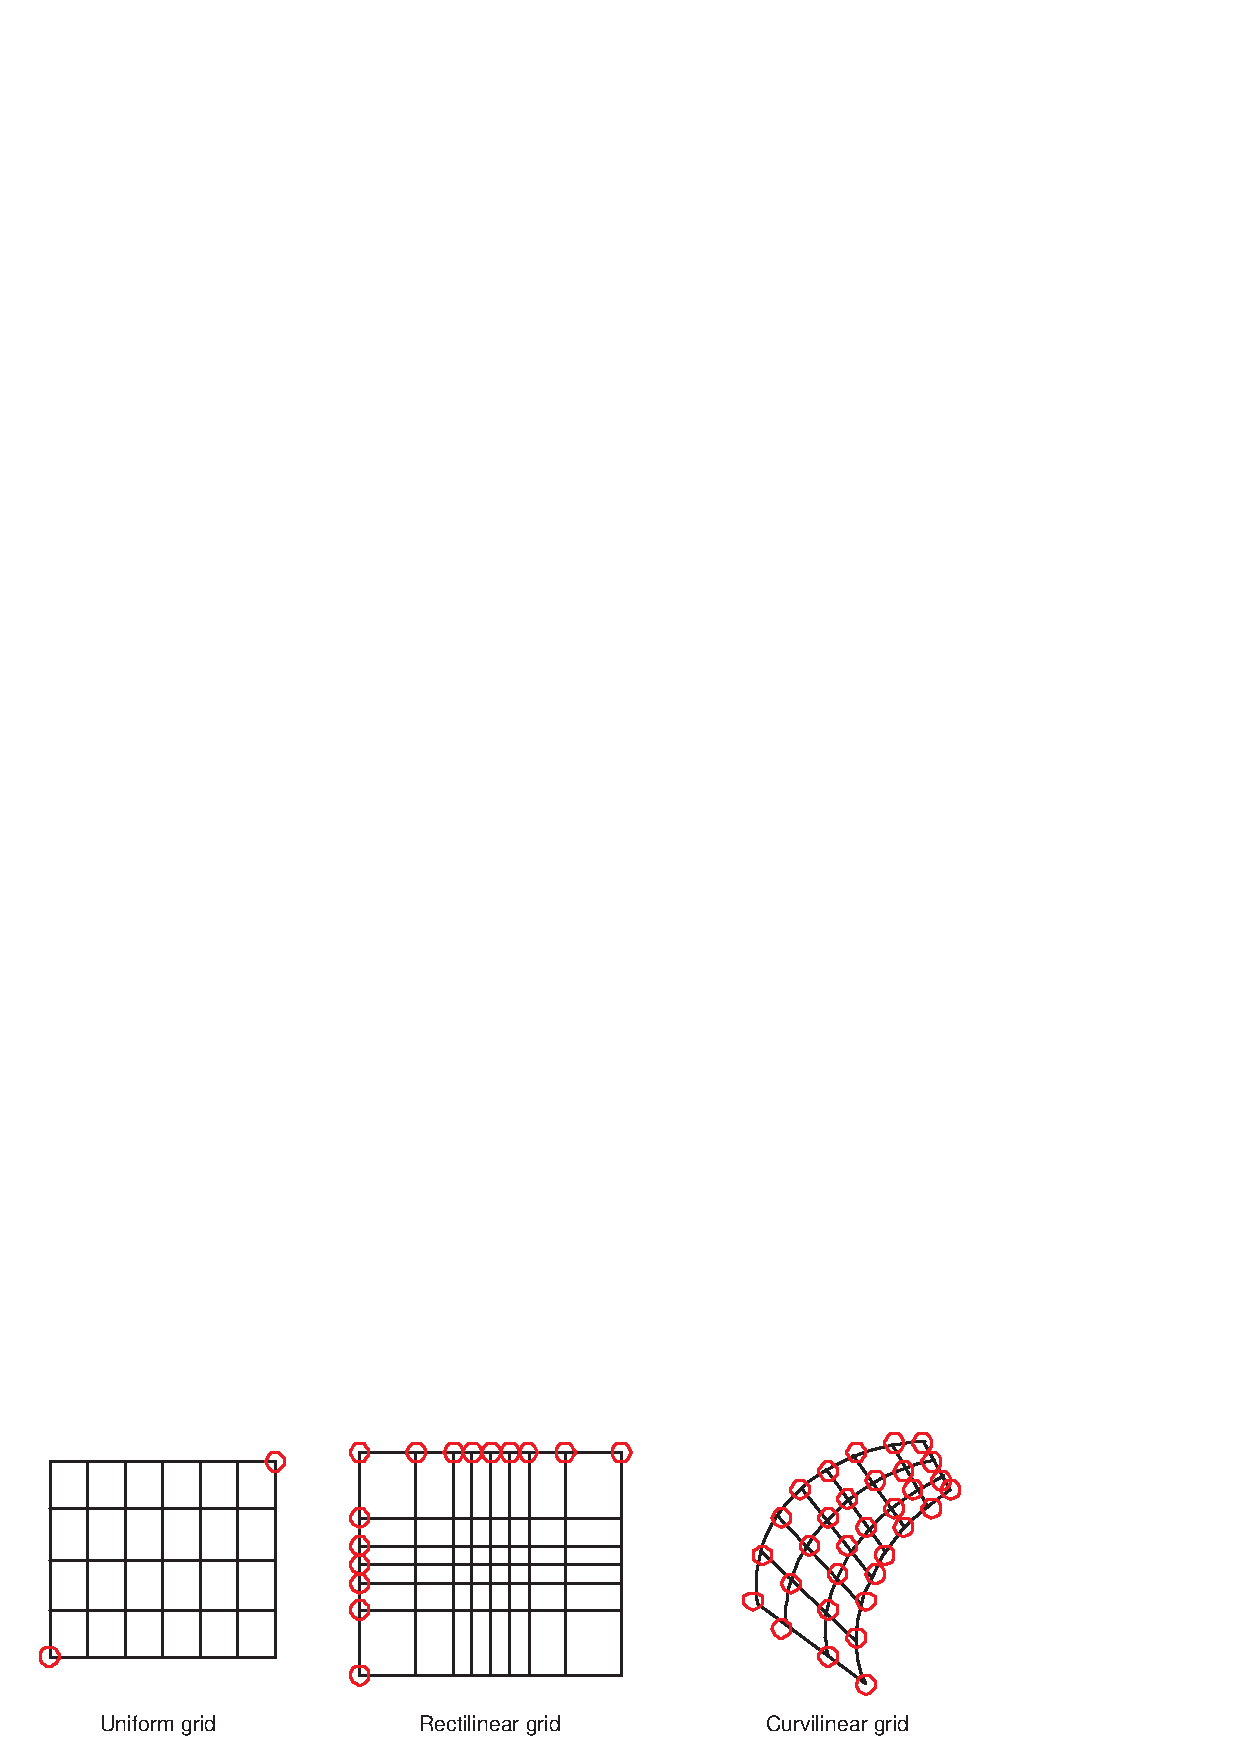
\includegraphics{LogRectGrids}}%
\lthtmlpictureZ
\lthtmlcheckvsize\clearpage}

\stepcounter{subsubsection}
\stepcounter{subsubsection}
\stepcounter{subsubsection}
\stepcounter{subsection}

\setlength{\parskip}{0pt}%

\setlength{\parskip}{0pt}

\setlength{\parindent}{0pt}%

\setlength{\parindent}{0pt}

\setlength{\baselineskip}{11pt}%

\setlength{\baselineskip}{11pt}
\stepcounter{subsection}
\stepcounter{section}
\stepcounter{subsection}
{\newpage\clearpage
\lthtmlinlinemathA{tex2html_wrap_inline1880}%
$10^{8}$%
\lthtmlinlinemathZ
\lthtmlcheckvsize\clearpage}

\stepcounter{subsubsection}
\stepcounter{subsubsection}
\stepcounter{section}
\stepcounter{subsection}
\stepcounter{subsubsection}
\stepcounter{subsubsection}
\stepcounter{subsection}
\stepcounter{section}
\stepcounter{subsection}
\stepcounter{subsection}

\setlength{\parskip}{0pt}%

\setlength{\parskip}{0pt}

\setlength{\parindent}{0pt}%

\setlength{\parindent}{0pt}

\setlength{\baselineskip}{11pt}%

\setlength{\baselineskip}{11pt}
\stepcounter{subsection}
\stepcounter{part}
\stepcounter{section}
\stepcounter{section}
\stepcounter{subsection}
{\newpage\clearpage
\lthtmlpictureA{tex2html_wrap5702}%
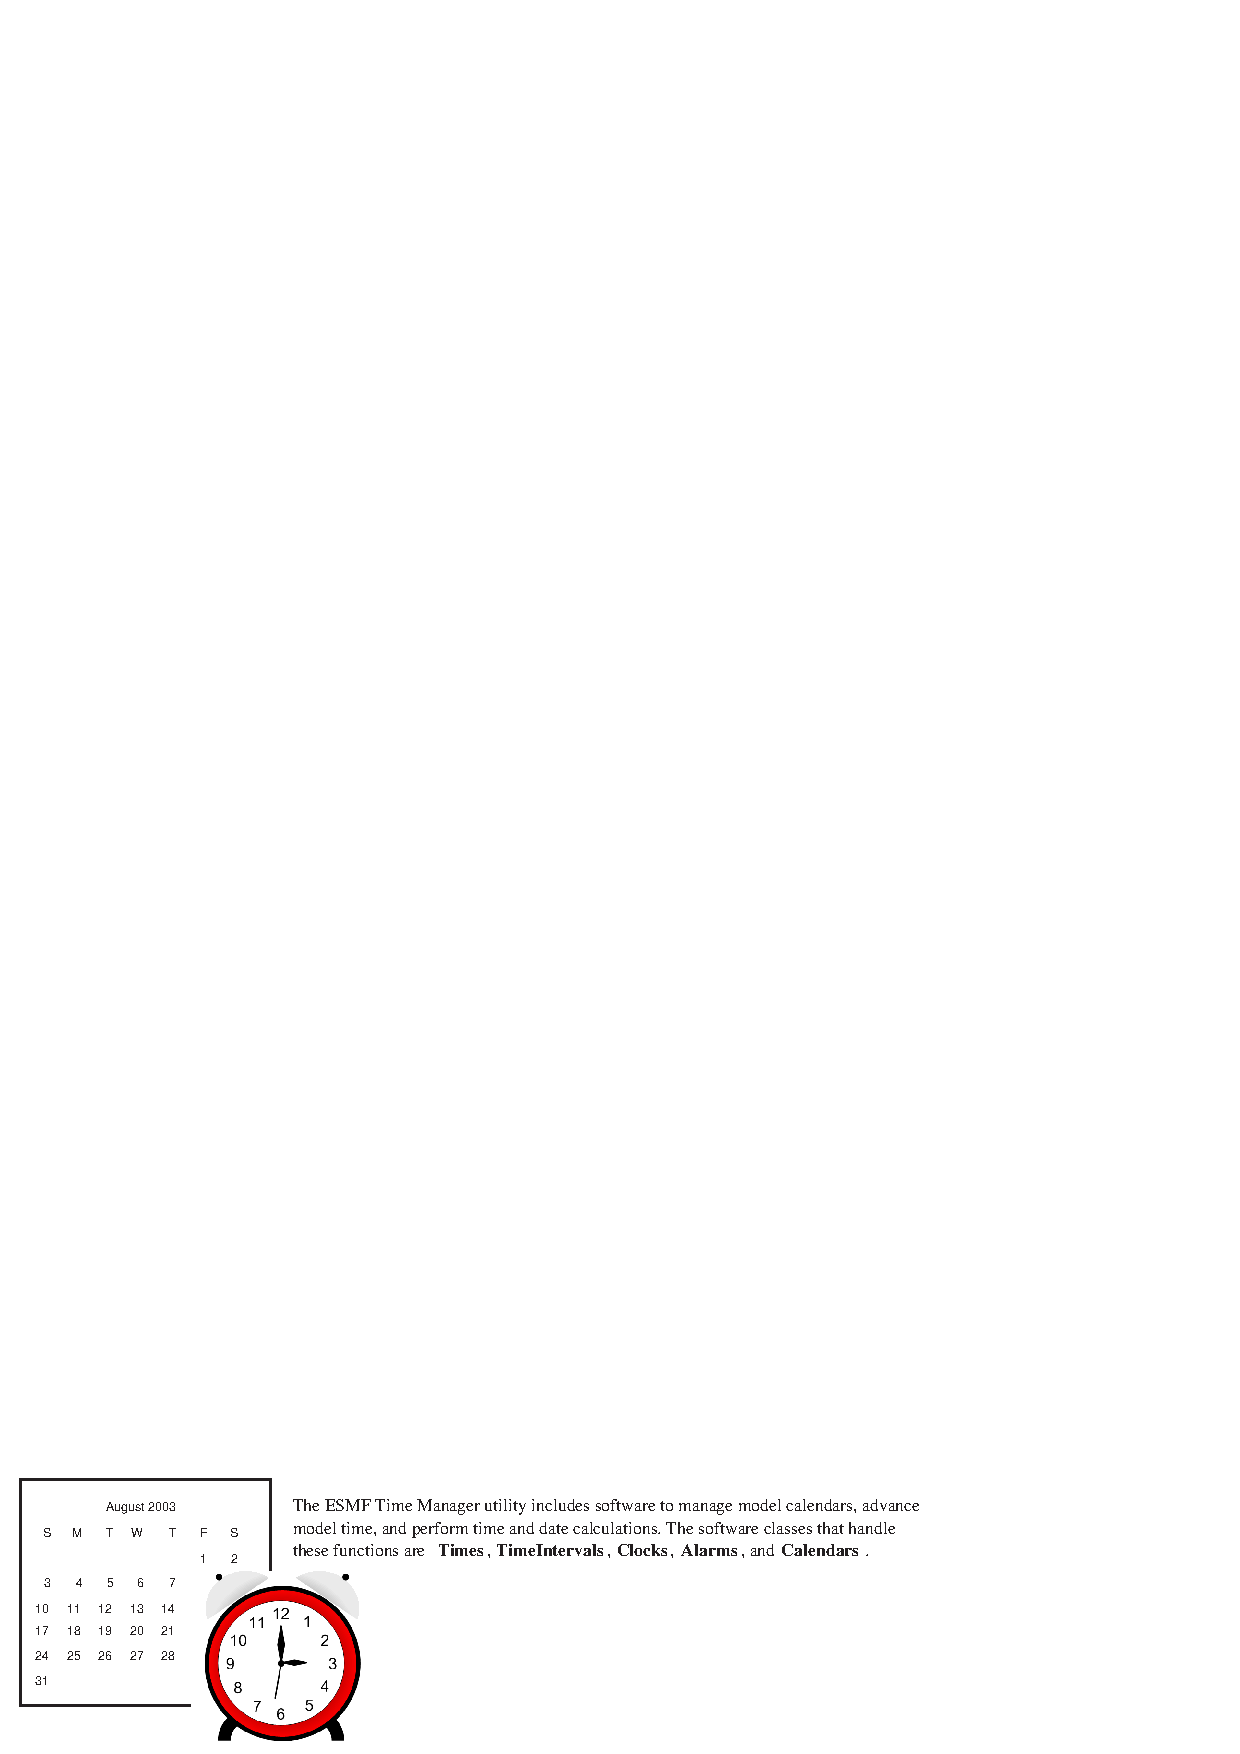
\includegraphics[]{TimeMgr_desc}%
\lthtmlpictureZ
\lthtmlcheckvsize\clearpage}

\stepcounter{subsection}
\stepcounter{subsection}
\stepcounter{subsection}
\stepcounter{section}
\stepcounter{subsection}
\stepcounter{subsection}

\setlength{\parskip}{0pt}%

\setlength{\parskip}{0pt}

\setlength{\parindent}{0pt}%

\setlength{\parindent}{0pt}

\setlength{\baselineskip}{11pt}%

\setlength{\baselineskip}{11pt}
\stepcounter{subsubsection}
\stepcounter{subsubsection}
\stepcounter{subsubsection}
\stepcounter{section}
\stepcounter{subsection}
\stepcounter{subsection}

\setlength{\parskip}{0pt}%

\setlength{\parskip}{0pt}

\setlength{\parindent}{0pt}%

\setlength{\parindent}{0pt}

\setlength{\baselineskip}{11pt}%

\setlength{\baselineskip}{11pt}
\stepcounter{subsection}
\stepcounter{section}
\stepcounter{subsection}
\stepcounter{subsection}

\setlength{\parskip}{0pt}%

\setlength{\parskip}{0pt}

\setlength{\parindent}{0pt}%

\setlength{\parindent}{0pt}

\setlength{\baselineskip}{11pt}%

\setlength{\baselineskip}{11pt}
\stepcounter{subsection}
\stepcounter{section}
\stepcounter{subsection}
\stepcounter{subsection}

\setlength{\parskip}{0pt}%

\setlength{\parskip}{0pt}

\setlength{\parindent}{0pt}%

\setlength{\parindent}{0pt}

\setlength{\baselineskip}{11pt}%

\setlength{\baselineskip}{11pt}
\stepcounter{subsection}
\stepcounter{section}
\stepcounter{subsection}
\stepcounter{subsection}
\stepcounter{section}
\stepcounter{subsection}
{\newpage\clearpage
\lthtmlinlinemathA{tex2html_wrap_inline2546}%
${\tt ESMF\_ConfigMod}$%
\lthtmlinlinemathZ
\lthtmlcheckvsize\clearpage}

\stepcounter{subsubsection}
\stepcounter{subsection}

\setlength{\parskip}{0pt}%

\setlength{\parskip}{0pt}

\setlength{\parindent}{0pt}%

\setlength{\parindent}{0pt}

\setlength{\baselineskip}{11pt}%

\setlength{\baselineskip}{11pt}
\stepcounter{subsection}
\stepcounter{section}
\stepcounter{subsection}
\stepcounter{subsection}

\setlength{\parskip}{0pt}%

\setlength{\parskip}{0pt}

\setlength{\parindent}{0pt}%

\setlength{\parindent}{0pt}

\setlength{\baselineskip}{11pt}%

\setlength{\baselineskip}{11pt}
\stepcounter{subsection}
\stepcounter{section}
\stepcounter{subsection}
\stepcounter{subsection}
\stepcounter{section}
\stepcounter{subsection}
\stepcounter{subsection}

\setlength{\parskip}{0pt}%

\setlength{\parskip}{0pt}

\setlength{\parindent}{0pt}%

\setlength{\parindent}{0pt}

\setlength{\baselineskip}{11pt}%

\setlength{\baselineskip}{11pt}
\stepcounter{subsection}
\stepcounter{section}
\stepcounter{part}
\stepcounter{section}
{\newpage\clearpage
\lthtmlpictureA{tex2html_wrap2960}%
\scalebox{0.8}{\includegraphics{Appendix_uml}}%
\lthtmlpictureZ
\lthtmlcheckvsize\clearpage}

\stepcounter{section}

\setlength{\parskip}{0pt}%

\setlength{\parskip}{0pt}

\setlength{\parindent}{0pt}%

\setlength{\parindent}{0pt}

\setlength{\baselineskip}{11pt}%

\setlength{\baselineskip}{11pt}

\end{document}
